% Customize font size as you wish 
\documentclass[11pt]{beamer} % Available font sizes are 8pt, 9pt, 10pt, 11pt, 12pt, 14pt, 17pt, 20pt.
% ********* DO NOT EDIT ********* %
\usepackage[utf8]{inputenc}
\usepackage{graphicx} % for including graphics
\usepackage{listings} % for including codes
%\usepackage{subfigure} % for including subfigures in a figure
%\usepackage{caption}
%\usepackage{subcaption}
\usepackage{multicol}
\usepackage{lmodern}
\usepackage{marvosym}
\usepackage{csquotes}
\usepackage{lipsum}
% ******************************* %

% Bibliography Settings %
% ------------- NOTE --------------- %
%     Editing is not recommended     %
% unless you know what you are doing %
% ---------------------------------- %
\usepackage[english]{babel}
\usepackage[
backend=biber,
citestyle=authortitle,
style=numeric,
natbib=true,
maxcitenames=2
]{biblatex}
% For tidiness, keeping fields of author, title, and year is recommended %
% Delete other fields of entries in ref.bib (Should have a more elegant way) %
\addbibresource{ref.bib}

% Theme & Font Preference
\usetheme{Berkeley}
\usecolortheme{seahorse}
%\usefonttheme[]{serif}

% Defined Commands %

% *************************** %

% Information to be included in the title page %
\title{ A Great Title }
\author{
A Famous Author \inst{1, 2, mystery} 
\and Another Famous Author \inst{2} }
\institute{
\inst{1} 
A Great Department \\
Beijing Normal University
\and 
\inst{2}
Another Great Department \\
Beijing Normal University
\and 
\inst{mystery} % the name for this entry can be anything
Somewhere unknown in the universe
}
\date{\today}

% Design
\logo{
    
\includegraphics[width=1.45cm,keepaspectratio]{design/BNU_logo.png}
% \includegraphics[height=1cm]{path/to/file/moreicons.png}
}

\begin{document}
\frame{\titlepage}

% Table of Contents
\AtBeginSection[] {
    \begin{frame}
    \frametitle{Table of Contents}
    \tableofcontents[currentsection] % parameter [currentsection] highlights the section about to start in the TOC, remove it if you dont like it
    \end{frame}
}

\section{Regular Frames}

\begin{frame}
    \frametitle{A Simple Frame}
    This is a regular frame, where you can see the items are shown together at once.
    \begin{itemize}
        \item item1
        \begin{itemize}
            \item nested item1.1
            \begin{itemize}
                \item I don't wanna stop
            \end{itemize}
            \item nested item1.2
            \begin{itemize}
                \item continue nesting ...
            \end{itemize}
        \end{itemize}
        \item I am here together with item1
    \end{itemize}
\end{frame}

\begin{frame}
    \frametitle{Animated Contents \& Items}
    The items in this frame will occur one by one. \pause
    \\ Now you'll see. \pause
    \begin{itemize}
        \item item1 goes first. \pause
        \item this is item2. \pause
        \item here comes item3.
    \end{itemize}
    \pause This is the end of the frame.
\end{frame}

\begin{frame}
    \frametitle{Highlighting}
    Example: \textbf{Inline Highlighting}

    % inline highlighting, use \alter{} command %
    My pitch is the most \alert{awesome} ever.

    % {block} is the environment and {Remark} is the title for the block
    \begin{block}{Remark} 
        \{block\} environment. This part of text is in a colored highlighting box.
    \end{block}
    %
    \begin{alertblock}{Important}
        \{alertblock\} environment means you ``alert'' the block, it turns out to be a color contrast the one used by the presentation. 
    \end{alertblock}

    \begin{examples}
        \{examples\} environment gives a color less contrasting to the one in presentation
    \end{examples}

\end{frame}

\begin{frame}[fragile] % when including codes, you have to use the [fragile] option parameter
    \frametitle{Insert Code}

    Here is how to insert codes in slides.

    \begin{lstlisting}[language=Python]
        import sys
        import numpy as np
        print('Hello World')
    \end{lstlisting}

    More details in \textbf{listings} documentations.

\end{frame}

\begin{frame}
    \frametitle{Insert Image}

    Single image insertion demo:
    
    \begin{figure}
        \centering
        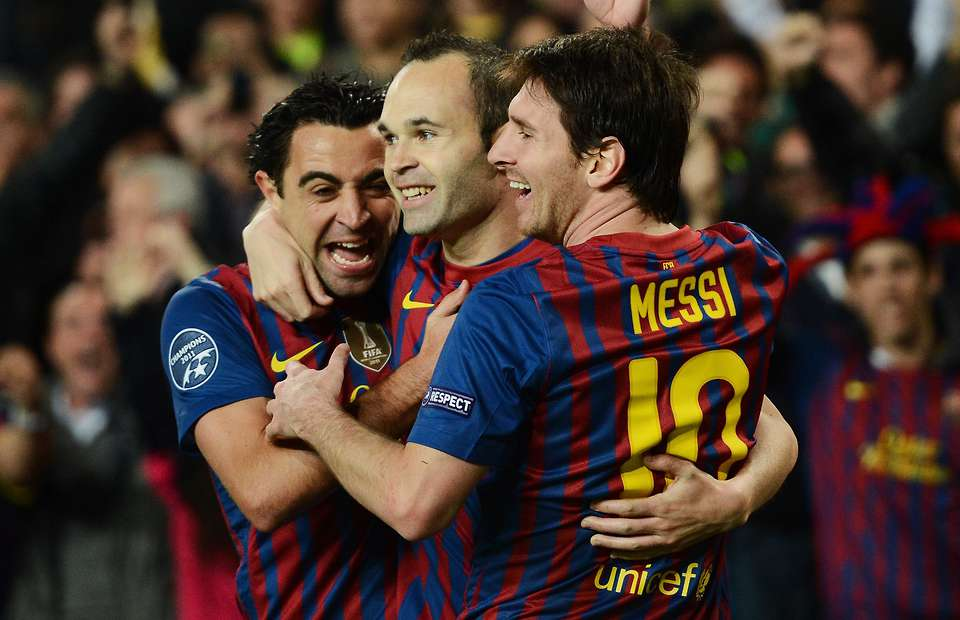
\includegraphics[width=0.8\textwidth]{imgs/golden-trio.jpg}
        \caption{FC Barcelona Golden Trio - Xavi, Iniesta, and Messi.}
        \label{fcb_golden_trio}
    \end{figure}

\end{frame}

\begin{frame}
    \frametitle{Multiple Image Insertion}

    2 in a row: (I think there will be a more elegant way...)
    \begin{columns}[t]
        \column{.5\textwidth}
        \centering
        \begin{figure}
            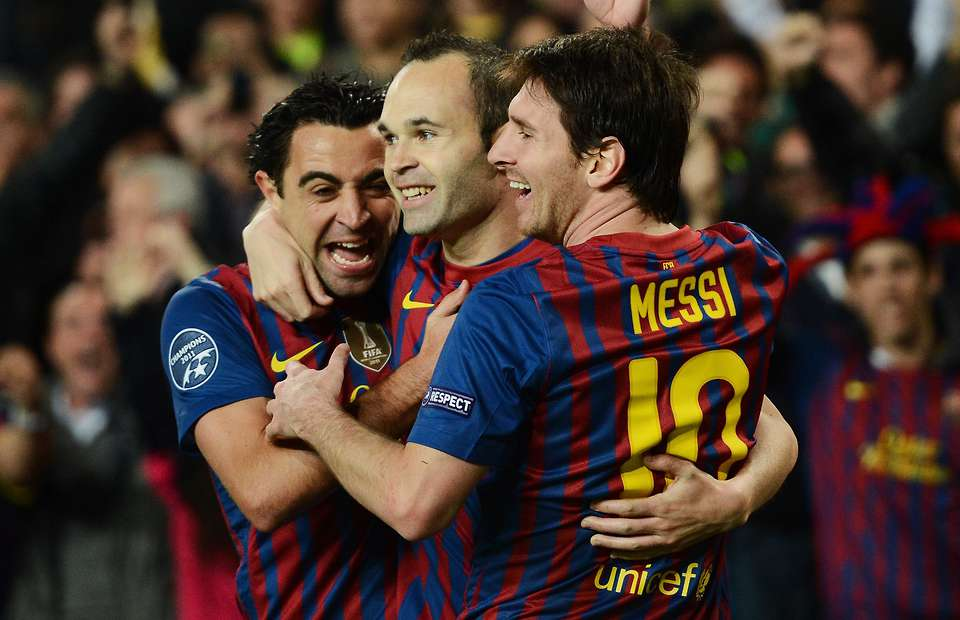
\includegraphics[width=\linewidth, height=.2\textheight, keepaspectratio]{imgs/golden-trio.jpg}
            \caption{Subfig 1}
        \end{figure}
        \begin{figure}
            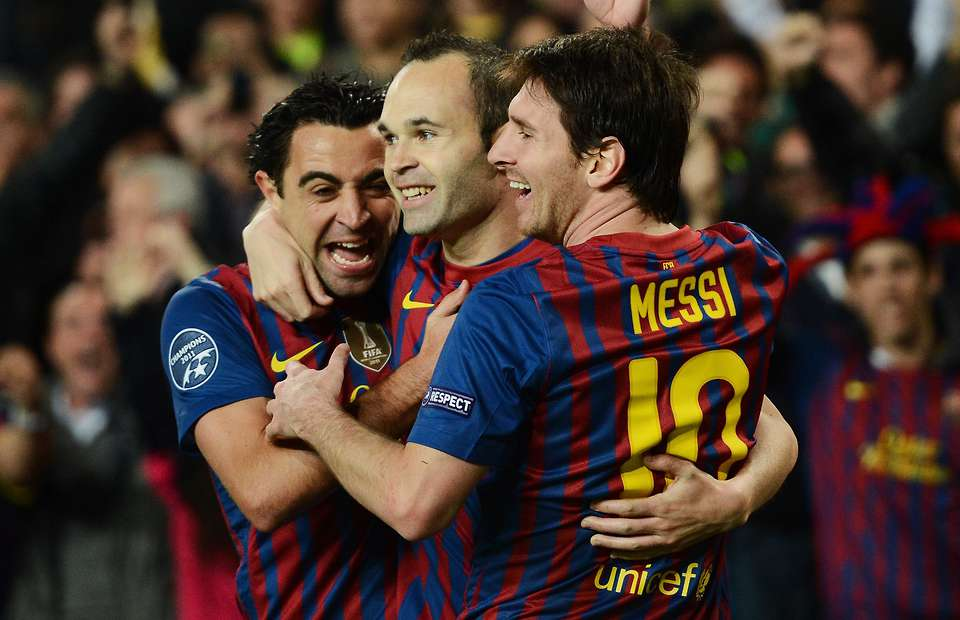
\includegraphics[width=\linewidth, height=.2\textheight, keepaspectratio]{imgs/golden-trio.jpg}
            \caption{Subfig 3}
        \end{figure}

        \column{.5\textwidth}
        \centering
        \begin{figure}
            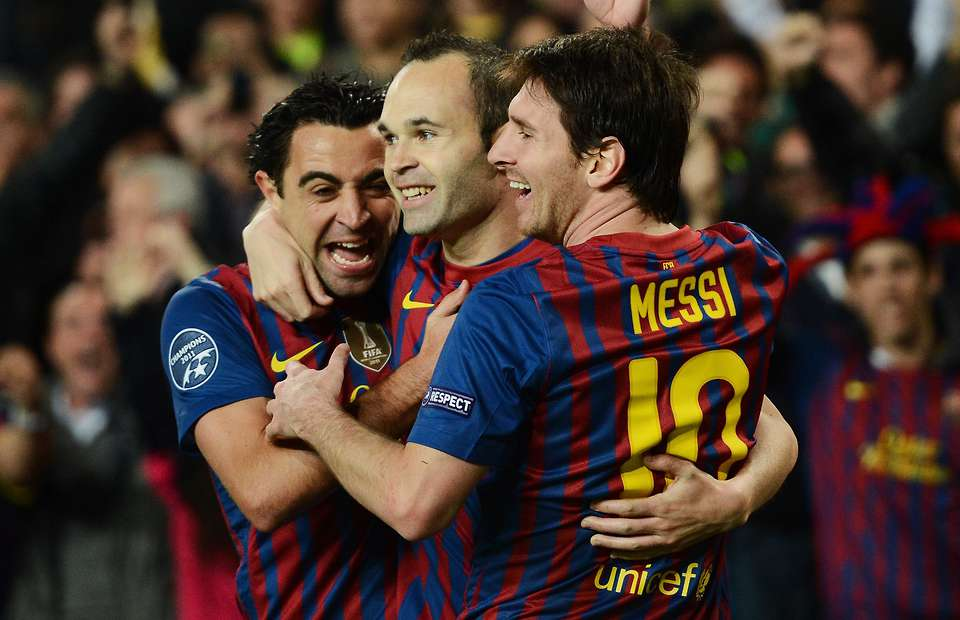
\includegraphics[width=\linewidth, height=.2\textheight, keepaspectratio]{imgs/golden-trio.jpg}
            \caption{Subfig 2}
        \end{figure}
        \begin{figure}
            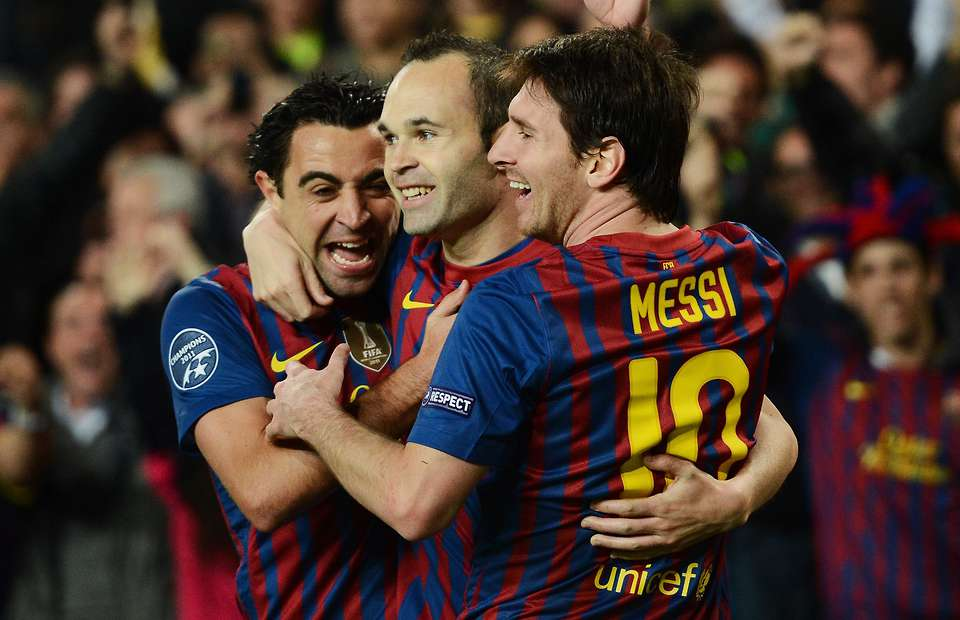
\includegraphics[width=\linewidth, height=.2\textheight, keepaspectratio]{imgs/golden-trio.jpg}
            \caption{Subfig 4}
        \end{figure}
    \end{columns}

\end{frame}

%******** does not work *********%
% \begin{frame}
%     \frametitle{An Alternative Approach}
% 
%     \begin{figure*}%加*的作用是跨栏(双栏和单栏latex的区别)
%         \centering
%         
%         %每列占整个文档的文本宽度的0.2,每列两张图像,两列图像,这些可以自行设置
%         \subfigure[the first subfigure]{
%         \begin{minipage}[b]{0.2\textwidth}
%         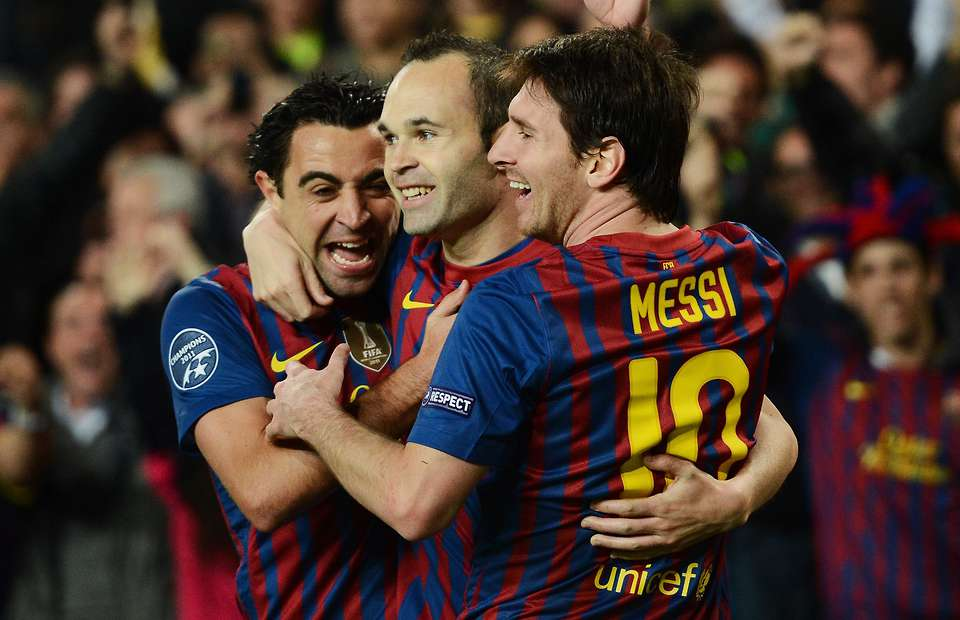
\includegraphics[width=\textwidth]{imgs/golden-trio.jpg} \\
%         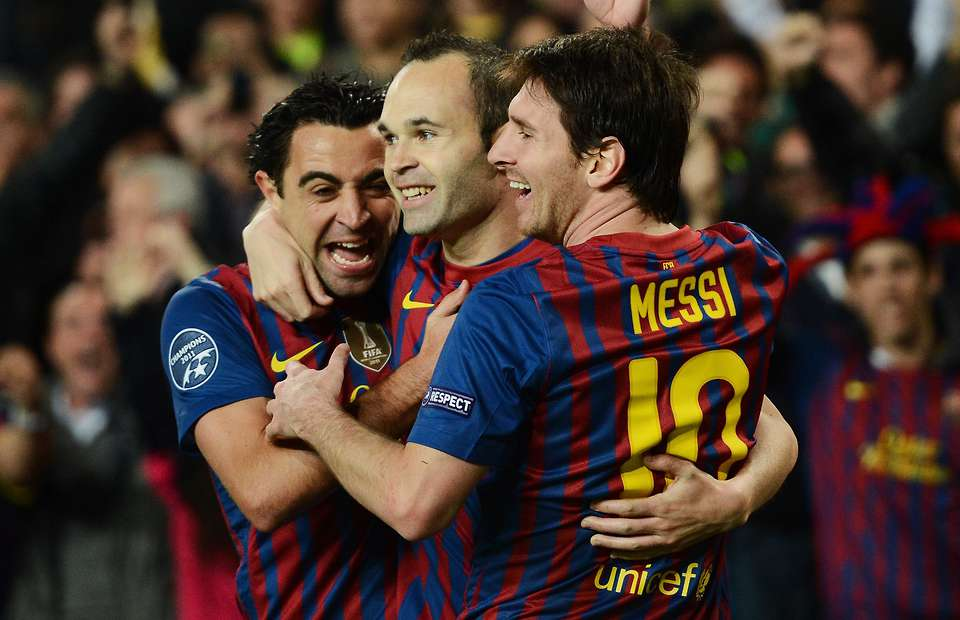
\includegraphics[width=\textwidth]{imgs/golden-trio.jpg}
%         \end{minipage}
%         }
%         \subfigure[the second subfigure]{
%         \begin{minipage}[b]{0.2\textwidth}
%         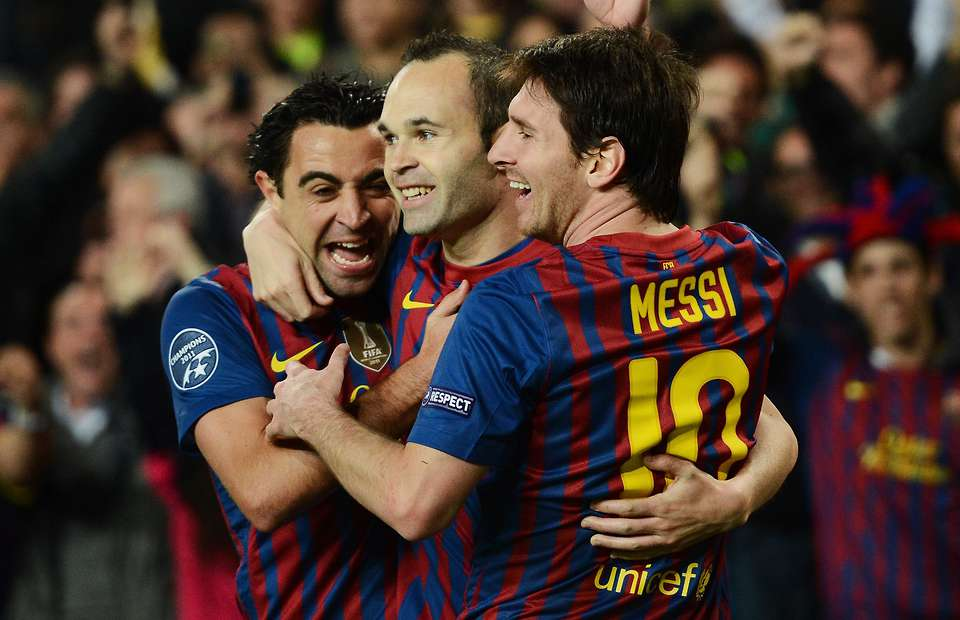
\includegraphics[width=\textwidth]{imgs/golden-trio.jpg} \\
%         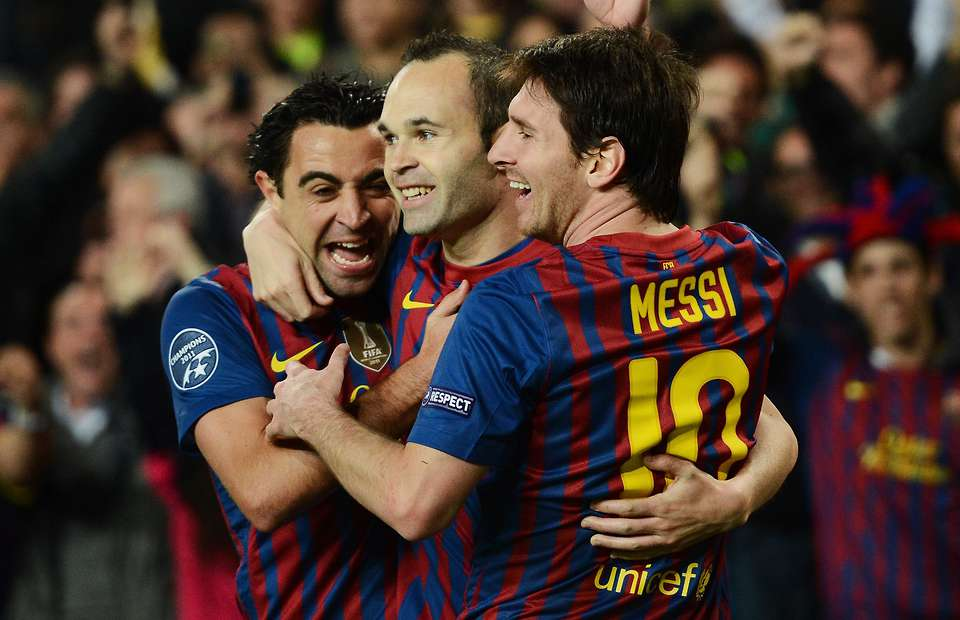
\includegraphics[width=\textwidth]{imgs/golden-trio.jpg}
%         \end{minipage}
%         }
%         \subfigure[the third subfigure]{
%         \begin{minipage}[b]{0.2\textwidth}
%         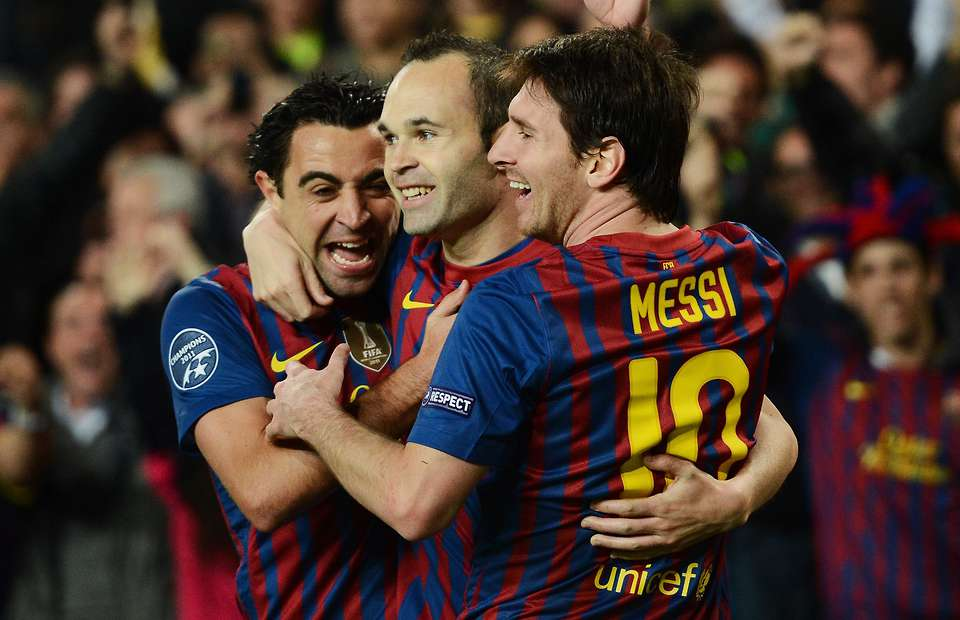
\includegraphics[width=\textwidth]{imgs/golden-trio.jpg} \\
%         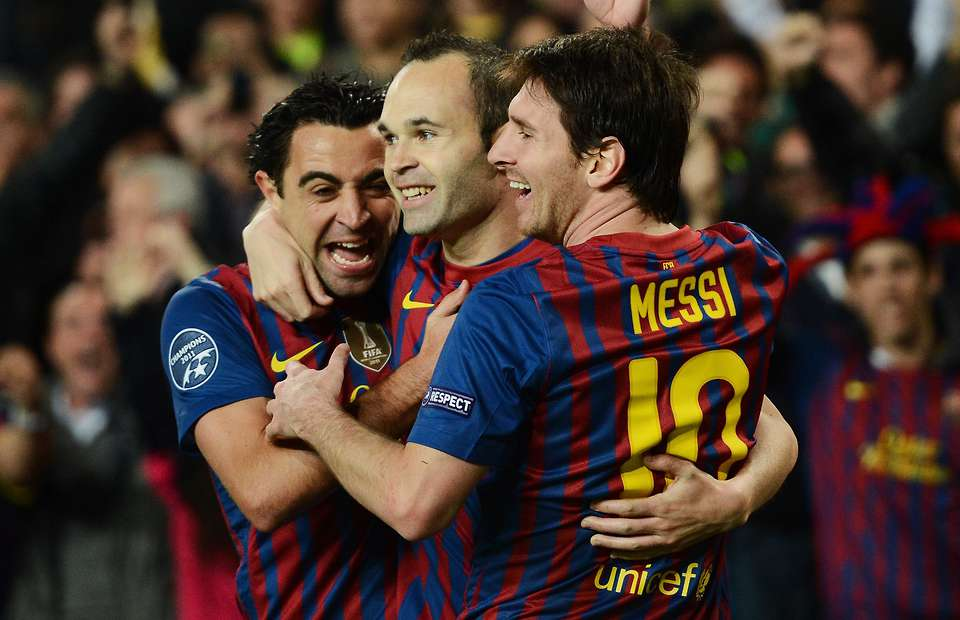
\includegraphics[width=\textwidth]{imgs/golden-trio.jpg}
%         \end{minipage}
%         }\caption{Figure caption}
%         \end{figure*}
% 
% \end{frame}

\section{Include Formulas}

\begin{frame}
\frametitle{Inline Formula}
    Use \alert{\$\dots\$} command to compose inline formulas.
    \begin{block}{Inline}
        Mass Energy Equivalence: $E=mc^2$ \\ 
        The area of a square is defined as $A=a^2$, where $a$ is the square's side.
    \end{block}
\end{frame}

\begin{frame}
    \frametitle{Numbered \& Unnumbered Formula Block}
    Numbered mass energy equivalence \& area of a square:
    \begin{equation}
        E = mc^2 
    \end{equation}
    \begin{equation}
        A = a^2
    \end{equation}

    Unnumbered version:
    \[E=mc^2\]
    \[A=a^2\]
    

\end{frame}

\section{Use Citations \& References}

\begin{frame}
    \frametitle{Citation}
    Yann LeCun's famous article \footfullcite{lecun2015deep}

    Aditya and Jure's famous article \footfullcite{grover2016node2vec}
\end{frame}

\begin{frame}
    \frametitle{Bibliography}
    \printbibliography
\end{frame}

\section{Ending}
\begin{frame}
    \frametitle{This is the end of the tutorial}
    You can find out more extended and advanced usages via Google, Overleaf, beameruserguide.pdf, StackExchange, and etc.

    For any issue, you are more than welcome to 
    \begin{itemize}
        \item Commit it at \href{https://github.com/htlee6/awesomeBNUbEAMer}{\underline{https://github.com/htlee6/awesomeBNUbEAMer}}
        \item Or send an email to \href{mailto:hauten.lee@mail.bnu.edu.cn}{\underline{hauten.lee@mail.bnu.edu.cn}} for contact
    \end{itemize}

\end{frame}

\end{document}